% TODO rimuovere
%\section{PNF + Metodologia Assurance}

\begin{frame}{Processo di Assurance e Proprietà}
  \begin{itemize}
    \item Necessità di un nuovo \alert{processo di assurance} per \alert{valutare} sistemi distribuiti su \alert{Proprietà Non Funzionali}
    
    \item \textbf{Verifiche di Assurance}: valutare se un sistema \alert{soddisfa i contratti} definiti, implicando la \alert{garanzia di \textbf{proprietà}} specifiche
    % i contratti sono soddisfatti
    % le proprietà sono garantire
    % soddisfando un requisito implica che ho una certa garanzia
    \begin{itemize}
      \item Valutazione \alert{continuativa}
      \item Valutazione \alert{su richiesta}
    \end{itemize}

    \item \textbf{Proprietà}: definiscono delle caratteristiche \alert{comportamentali} del sistema \textit{(Scalabilità, Affidabilità, Confidenzialità, Integrità, Disponibilità, ...)}

  \end{itemize}
\end{frame}


\begin{frame}{Metodologia di Assurance}
  \begin{columns}
    \begin{column}{.6\textwidth}
      \begin{itemize}%[<+->]
        \item \textbf{Metriche}: misurano gli \alert{stati} rilevanti del sistema

        \item \textbf{Evidence}: \alert{dati} raccolti dalle metriche, utilizzati come \alert{prove per i contratti} 
        
        \item \textbf{Contratti}: \alert{verificano} formalmente la validità di \alert{PNF} 

        \item \textbf{Report}: lista delle \alert{proprietà valutate} con il \alert{relativo esito} e le evidence a supporto

      \end{itemize}
      \vspace{1em}
    \end{column}

    \begin{column}{.4\textwidth}
      \centering
      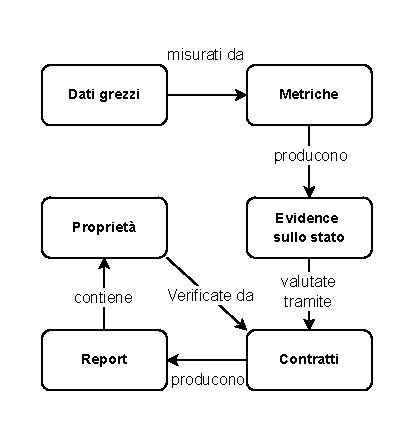
\includegraphics[width=\textwidth]{assets/metriche-contratti.drawio.pdf}
    \end{column}

  \end{columns}
\end{frame}
